\section{Stage 1: Program Generator} \label{sec:work_stage1_program_generator}

\begin{figure}[htbp]%[H]
  \centering
  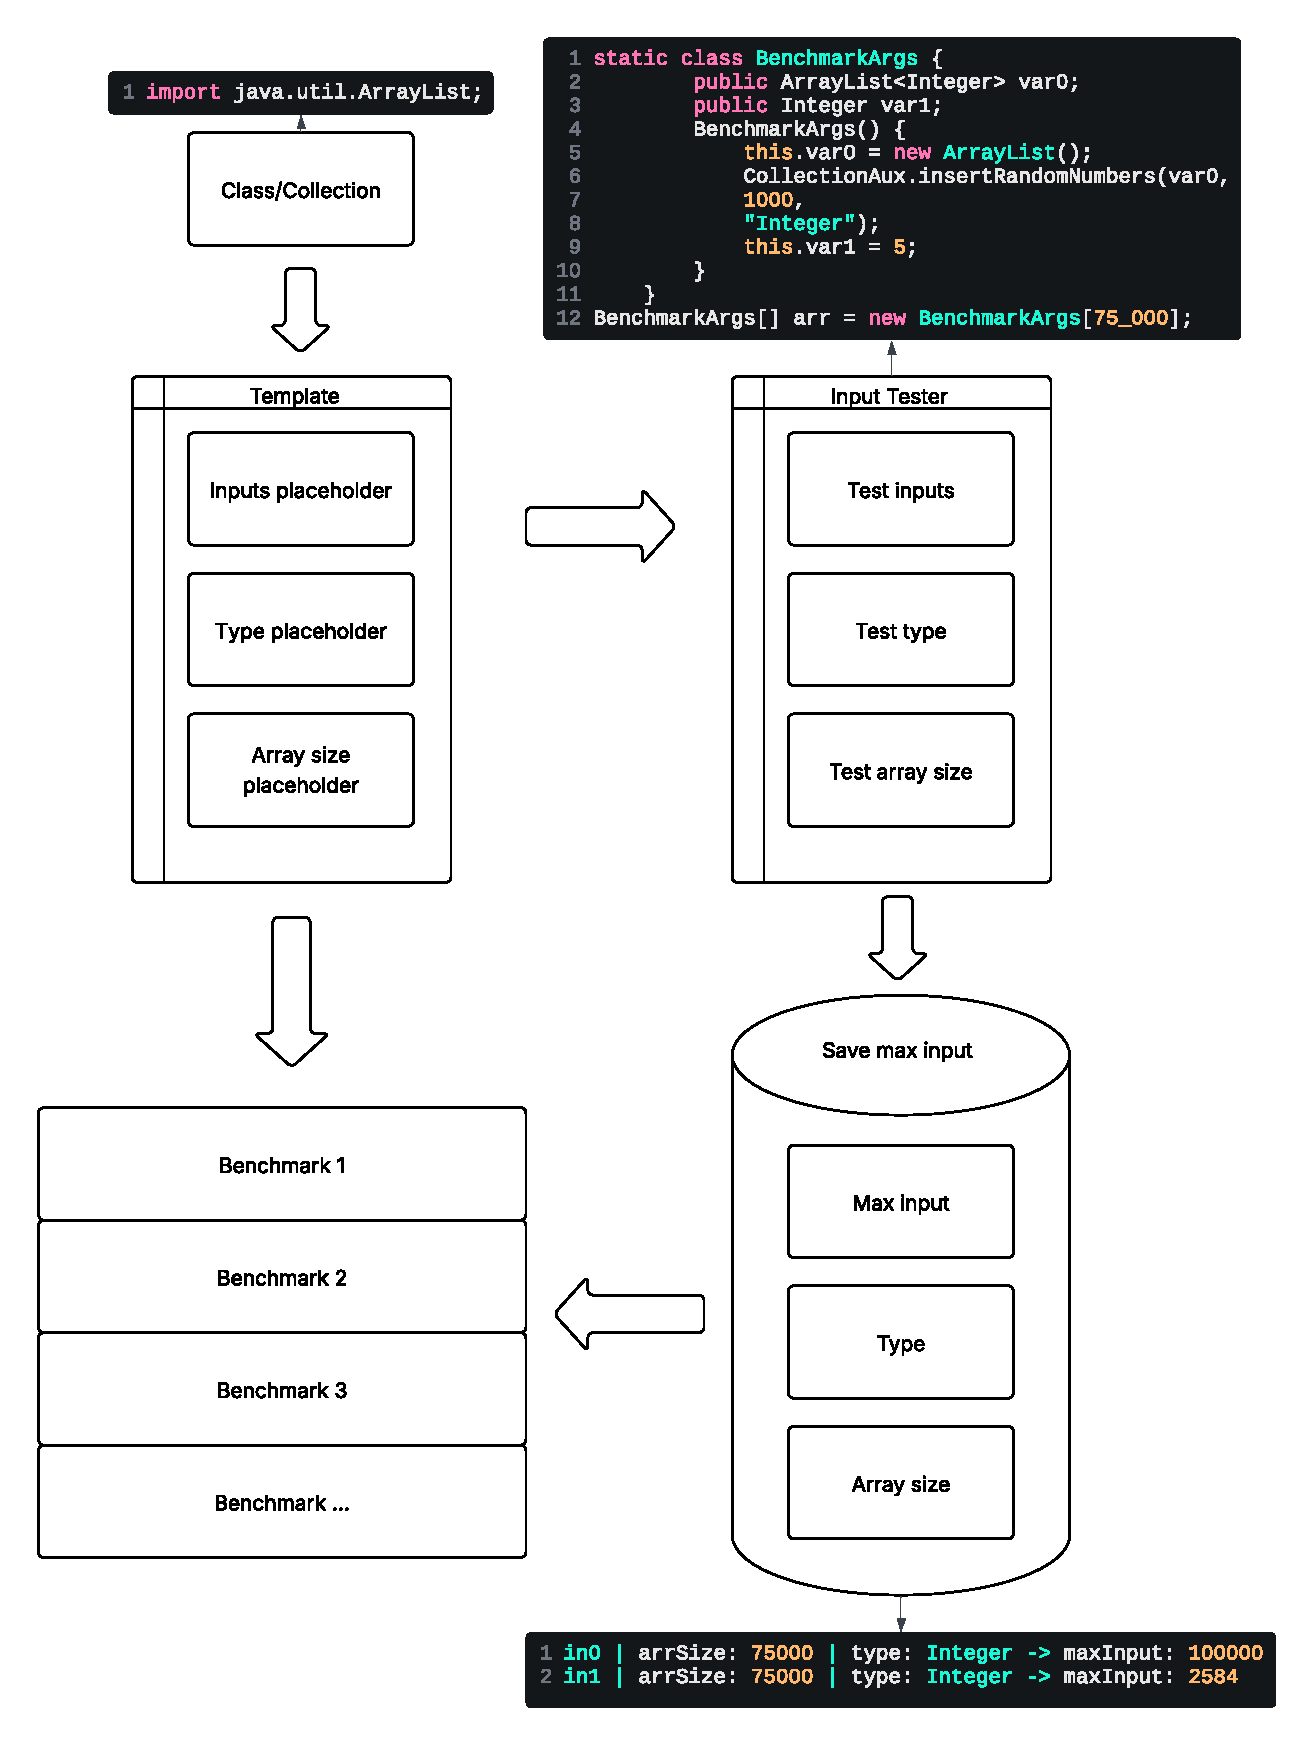
\includegraphics[width = 1 \textwidth]{figures/program_generator.pdf}
  \caption{Program Generator}
  \label{fig:program_generator}
\end{figure}

In order to be able to predict energy using ML models it is of course needed a lot of data, so the models can train, and the results can be analyzed. To obtain a considerable amount of data, a program generator was built, as illustrated in Figure~\ref{fig:program_generator}.

The program generator works alongside with Java Spoon to make it the more general as possible allowing custom programs to be mass generated.
The generator works for custom, developer-created, Java classes, for most collections interface (Lists, Sets, Maps) implementations, for utility classes like Math, Base64, Duration, and it can be called to analyze all the public methods of the class or just specific ones.

\subsection{Template Creation} \label{sec:work_stage1_template_creation}

%\FloatBarrier

%\begin{listing}[htbp]
%\begin{minted}[linenos, fontsize=\small, frame=none, bgcolor=white,breaklines=true,breakanywhere=true]{java}
%
%public class ArrayList_add_java_lang_Object_ {
%    public static void main(String[] args) throws Exception {
%        int iter = 0;
%        try {
%            BenchmarkArgs[] arr = new BenchmarkArgs["numberOfFunCalls"];
%            populateArray(arr);
%            TemplatesAux.sendStartSignalToOrchestrator(args[0]);
%            TemplatesAux.launchTimerThread(1100);
%            iter = computation(arr, arr.length);
%        } catch (OutOfMemoryError e) {
%            TemplatesAux.writeErrorInFile("ArrayList_add_java_lang_Object_", "Out of memory error caught by the program:\n" + e.getMessage());
%        } catch (Exception e) {
%            TemplatesAux.writeErrorInFile("ArrayList_add_java_lang_Object_", "Error caught by the program:\n" + e.getMessage());
%        } finally {
%            TemplatesAux.sendStopSignalToOrchestrator(args[0], iter);
%        }
%    }
%
%    static class BenchmarkArgs {
%        public ArrayList<changetypehere> var0;
%
%        public changetypehere var1;
%
%        BenchmarkArgs() {
%            this.var0 = new ArrayList();
%            CollectionAux.insertRandomNumbers(var0, "ChangeValueHere1_changetypehere", "changetypehere");
%            this.var1 = "ChangeValueHere2_changetypehere";
%        }
%    }
%
%    private static void arrayList_add_java_lang_Object_(ArrayList var, changetypehere arg0) {
%        var.add(arg0);
%    }
%
%    private static int computation(BenchmarkArgs[] args, int iter) {
%        int i = 0;
%        while (!TemplatesAux.stop && i < iter) {
%              arrayList_add_java_lang_Object_(args[i].var0, args[i].var1);
%               i++;
%        }
%        return iter;
%    }
%
%    private static void populateArray(BenchmarkArgs[] arr) {
%        for (int i = 0;i < "numberOfFunCalls";i++) {
%          arr[i] = new BenchmarkArgs();
%        };
%    }
%
%    private String input1 = "ChangeValueHere1";
%    private String input2 = "ChangeValueHere2";
%}
%
%
%\end{minted}
%\caption{Example of template for List.add(Object)}            
%\label{lst:template_example}
%\end{listing}

The first step to generate multiple programs is to first create an intermediate template capable of holding the necessary code that will later be used for energy profiling.

The program generator starts by reading a custom Java file (or just access the Lists, Sets, Maps classes), and using Spoon it finds every public method available in the provided class. If it is needed to analyze a specific method, the generator will search in the class for every method with the name requested. Then it has access to all the public methods in the class and what parameters they receive.
Since it has access to the whole custom class, it can see how its constructors are called, and use them if any of the methods parameters requires. It recursively calls constructors if needed, making it very versatile to use. 

After identifying the methods that will be targeted, it starts by creating templates for each of them. 

Template important features:

\begin{itemize}

  \item Input placeholders: Placeholders that will be later changed with real values for inputs, in this case inputs are variable values. 

  \item Type placeholder: Placeholders that will later be replaced with Java wrapper classes.
  
  \item Array Size placeholder: Placeholder that will later be replaced with the value of an array size. (This array will be explained in \ref{sec:work_stage2_orchestrator}). 

\end{itemize}

Also, the template is structured so that the programs will work in harmony with the Orchestrator, that will extract the energy profile for each program (see Section~\ref{sec:work_stage2_orchestrator}), so when the placeholders are replaced with actual values, the orchestrator can run the program, and communicate with them.


\begin{listing}[H]
\noindent\rule{\linewidth}{0.4pt}
\begin{minted}[linenos, fontsize=\small, frame=none, bgcolor=white,breaklines=true,breakanywhere=true]{java}
static class BenchmarkArgs {
        public ArrayList<changetypehere> var0;

        public changetypehere var1;

        BenchmarkArgs() {
            this.var0 = new ArrayList();
            CollectionAux.insertRandomNumbers(var0, "ChangeValueHere1_changetypehere", "changetypehere");
            this.var1 = "ChangeValueHere2_changetypehere";
        }
    }
\end{minted}
\noindent\rule{\linewidth}{0.4pt}
\caption{Example of variable placeholders creations}            
\label{lst:var_placeholders}
\end{listing}

The template creates a class that holds the necessary variables the method needs to run, Listing~\ref{lst:var_placeholders} shows an example of the variables that need to be created to run the method \texttt{List.add(Object)}. First it creates the list with the smallest constructor possible, then if the variable is a collection (List, Set, Map) it calls a custom-made method that populates collections with random values of a given type, and then it starts creating variables of parameters that the method \texttt{List.add(Object)} uses. The placeholder \texttt{ChangeValueHere1} will change to a random number, it contains a number \texttt{1} because it represents the input number of the method that will later help the model training understand how inputs can affect energy consumption. The placeholder \texttt{changetypehere} later changes to a type. The template after the transformation can be seen in the Listing~\ref{lst:var_placeholders_replaced}


\begin{listing}[H]
\noindent\rule{\linewidth}{0.4pt}
\begin{minted}[linenos, fontsize=\small, frame=none, bgcolor=white,breaklines=true,breakanywhere=true]{java}
static class BenchmarkArgs {
        public ArrayList<Integer> var0;

        public Integer var1;

        BenchmarkArgs() {
            this.var0 = new ArrayList();
            CollectionAux.insertRandomNumbers(var0, 1000, "Integer");
            this.var1 = 10;
        }
    }
\end{minted}
\noindent\rule{\linewidth}{0.4pt}
\caption{Example of variable placeholders replaced}            
\label{lst:var_placeholders_replaced}
\end{listing}


It is worth mentioning that the types used by the generator are the Java wrapper classes, which are object representations of the primitive types. Using these types it is possible to achieve a more general generator, as every program can use them and if other custom types were used it would make the generator more complex and not general.

What mostly differs from template to template is the number of variables used, because different methods have different parameters, so the template can have more or less input placeholders, also the type placeholder changes according to the methods types and parameters.


Creating the template for each method allows cutting off time of the program generation by only having to replace values of the placeholders instead of needing to create the whole program all over again, since the programs for the same method only differ in inputs, types and array size, maintaining all the structure.

\subsection{Input Tester} \label{sec:work_stage1_input_tester}

A very important aspect of the program generator is the inputs it generates. Every method works differently, receives different parameters, and even when changing the values of these parameters, the method can behave completely different. So, this generator has an intermediate step, between the creation of the template and creating multiple programs, it finds the maximum size the input parameters should receive. Knowing the maximum size the different parameters can have is very important as it needs to be big enough, so the energy profiles can be abundant, but not to big so that the programs start to get out of memory or taking too much time to complete.
The input search works by using binary search. It has limits on the inputs (1-100,000) and it starts by trying to run the program with the half of the max input which is 50,000. Then it runs the program for maximum of 10 seconds, which is a threshold based on empirical experimentation, and waits for the exit code of the program, if it is an error code it will lower the input by half again, of it is a normal finish code, it will increase the input by half. This operation is done until the maximum value for the input is found. If the method that is being tested has more than one input, the input tester, first sets all the input values to 1 and then starts the binary search individually for each of the parameters one by one while leaving the other parameters with the value of 1. This avoids having to find multiple combinations of parameters which would increase the time complexity exponentially. Since the process of finding the max inputs is time-consuming, when the maximum value is found, the values of the input type, maximum value and order (if it was the parameter 1 or parameter 2 or parameter 3) are stored in a file, so if the actual programs later generated are not stored, using this files they can be quickly generated. It is worthy to mention that the maximum inputs found depend heavily on the machine where the program generation is taking place, as different hardware will change the maximum values allowed for the inputs.

\begin{tcolorbox}[
    title=Example: Input Testing Process for \texttt{List.add(index, Element)},
    colback=gray!5!white,
    colframe=gray!75!black,
    fonttitle=\bfseries,
    breakable,
    label={box:add-method-testing}
]

Consider analyzing the \texttt{add} method of a list with the following parameters:
\begin{itemize}
    \item \texttt{arg0}: Size of the list (integer)
    \item \texttt{arg1}: Index at which to insert the new value (integer)
    \item \texttt{arg2}: Value to be added (integer)
\end{itemize}

\textbf{Step 1 – Varying \texttt{arg0} (list size):}

\begin{itemize}
    \item Iteration 1: \texttt{arg0 = 25,000}, \texttt{arg1 = 1}, \texttt{arg2 = 1}
    \item Iteration 2: \texttt{arg0 = 12,500}, \texttt{arg1 = 1}, \texttt{arg2 = 1}
    \item Iteration 3: \texttt{arg0 = 6,250}, \texttt{arg1 = 1}, \texttt{arg2 = 1}
    \item $\vdots$
    \item Final Iteration: \texttt{arg0 = 1,700}, \texttt{arg1 = 1}, \texttt{arg2 = 1}
\end{itemize}

\textbf{Step 2 – Varying \texttt{arg1} (index):}

\begin{itemize}
    \item Iteration 1: \texttt{arg0 = 1}, \texttt{arg1 = 25,000}, \texttt{arg2 = 1}
    \item Iteration 2: \texttt{arg0 = 1}, \texttt{arg1 = 12,500}, \texttt{arg2 = 1}
    \item $\vdots$
    \item Final Iteration: \texttt{arg0 = 1}, \texttt{arg1 = 1}, \texttt{arg2 = 1}
\end{itemize}

{Note: Since the list size (\texttt{arg0}) remains 1, the maximum valid index (\texttt{arg1}) is constrained to 1. This reveals a limitation in the input testing approach.}

\textbf{Step 3 – Varying \texttt{arg2} (value to be added):}

\begin{itemize}
    \item Iteration 1: \texttt{arg0 = 1}, \texttt{arg1 = 1}, \texttt{arg2 = 25,000}
    \item Iteration 2: \texttt{arg0 = 1}, \texttt{arg1 = 1}, \texttt{arg2 = 37,500}
    \item $\vdots$
    \item Final Iteration: \texttt{arg0 = 1}, \texttt{arg1 = 1}, \texttt{arg2 = 100,000}
\end{itemize}

\textbf{Final stored input limits:}
\begin{itemize}
    \item \texttt{arg0} — \texttt{integer} — \texttt{1,700}
    \item \texttt{arg1} — \texttt{integer} — \texttt{1}
    \item \texttt{arg2} — \texttt{integer} — \texttt{100,000}
\end{itemize}

\end{tcolorbox}


The fact that the input has a range of 1 to 100,000 it allows using binary search which makes the search much faster than linear search.
Nevertheless, the input search does not come without some limitations. First it is constrained to identifying valid input values within the range of 1 to 100,000. Throughout this project we dealt frequently with lists and collections, which require a minimum size of 1 to function correctly. Although this value can be changed in the future, for now it ensures compatibility with most common data structures. The higher bound of 100,000 was chosen due to practical experience, as larger input values would lead to higher execution times and memory crashes. Another limitation is on how the input handles multiple parameter methods. During its search for a valid input, it needs to fix all the other parameters that is not searching, with a default value (typically 1). This approach simplifies the testing process and improves efficiency by avoiding the exponential complexity of testing all possible parameter combinations. However, it will introduce limitations in cases where the parameters are interdependent, which can lead to not estimating the real highest input possible. The process also has a timeout of 10 seconds. This threshold was empirically selected to balance precision and practicality, based on our needs and available hardware.
Despite these limitations, the input search plays a crucial role in ensuring that the program generator produces viable test cases. By identifying input ranges that are both valid and computationally achievable, it reduces the unusable generated programs (e.g., due to timeouts or crashes), and maximizing the number of generated programs, that can be used for energy profiling.



\subsection{Program Generation} \label{sec:work_stage1_program_generation}

Finally, when the templates are created, and the maximum inputs are found the program generation can finally begin. This part consists on picking every template created and replacing the placeholder values with actual values created by a random number generator.

It starts by looping through the types and changing them to the Java wrapper classes, then it loops through the array size. Lastly, it loops through the input sizes determined by the input tester and can repeat this process a configurable number of times. By increasing the number of iterations, results in more programs being generated with random inputs, constrained by the previously identified input bounds.

This process easily generate thousands of programs which are crucial to train machine learn models that are able to predict energy consumption. When generating programs, a number is chosen to balance the requirements for effective model training while minimizing the time spent on input testing and collecting energy profiles. Afterwards, that the programs are ready to be compiled and used.